\section{Introduction}
\label{sec:intro}

Referring-expression comprehension usually assumes that every expression
denotes exactly one object in the image.  A deployed system cannot rely on
this assumption: a request may be invalid, stale, or unsupported by the
current scene, and the system must decide whether to localize or abstain.
Generalized referring-expression benchmarks make absence explicit by
including no-target cases~\cite{ding2026grex}.  The practical problem is
therefore not only to predict a box, but to emit a box \emph{selectively}.

Detector-style grounding models expose text-conditioned queries and matching
scores~\cite{liu2025groundingdino}.  In practice, a score is often asked to do
three jobs: filter category-ineligible candidates, order the remaining
instances by the complete expression, and determine whether any candidate
should be accepted.  These jobs have different semantics.  \emph{Admission}
constructs a comparison set, \emph{Ranking} is relative within that set, and
\emph{Rejection} is a sample-level decision.  A ranker must always choose a
winner, even when every candidate is invalid; a rejector must instead suppress
the entire sample.  Coupling these decisions is consequently an optimization
problem rather than a naming inconvenience, as the cases in
Fig.~\ref{fig:teaser} illustrate.

We begin from a frozen, data-finetuned Grounding DINO representation.  Across
26,488 validation expressions per seed, its all-query geometry contains an
IoU$\geq0.5$ candidate in every case.  Admission removes the final compatible
candidate in only 0.31--0.38\% of examples, yet 27.23--27.39\% remain ranking
errors inside the eligible set.  A shared-scalar Admission/Rejection control
exposes a second failure: the two gradients have negative mean cosine in all
three seeds.  Separate outputs over the same trainable feature owner barely
change calibration FPR95, whereas disjoint owners improve rejection without
changing the localization route.

We therefore introduce \method: \textbf{Admission, Ranking, and Rejection with
Ownership-Separated Weights}.  A frozen generator supplies candidates.
Admission uses an optional category cue to construct an eligible set.  The
complete expression ranks candidates within that set.  An independent
sample-level score then accepts or rejects the result.  Every deployed surface
has an exclusive trainable owner.  A dashed auxiliary route can carry
Admission supervision during training, but it never enters a deployed decision
score and cannot become a hidden fourth score.  \arrowv uses a visual support exemplar;
\arrowt uses an explicit canonical category phrase without a visual support
image; \arrown is a category-agnostic mechanism control.  The category cue is
separate from the complete expression that still owns geometry and Ranking.

\begin{figure*}[t]
  \centering
  \IfFileExists{figures/fig1_teaser.pdf}{%
    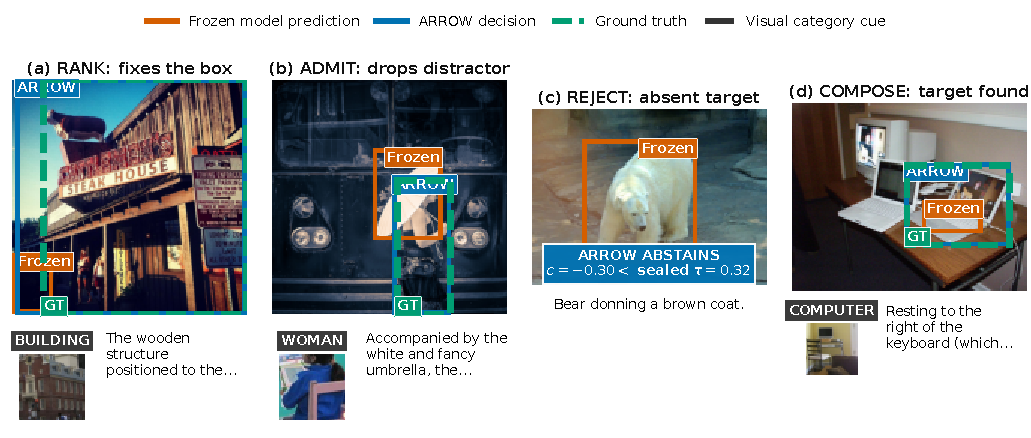
\includegraphics[width=\textwidth]{figures/fig1_teaser.pdf}%
  }{\fbox{\parbox[c][1.15in][c]{0.96\textwidth}{\centering
    Deterministically selected candidate, Admission, and no-target examples
    will be generated from sealed records.}}}
  \caption{A valid candidate may already exist; reliable grounding must learn
  who enters, who wins, and whether any winner should be emitted, without
  allowing the three duties to overwrite one another.  Zero-training examples
  are selected from sealed records by deterministic predicates; panel (d)
  adds a level-3 compositional success.  Failure cases remain in the
  qualitative supplement.  Detached cue tiles
  below panels (a), (b), and (d) are external Admission inputs, not crops from
  the evaluated detection image.}
  \label{fig:teaser}
\end{figure*}

Our evidence supports three claims.  First, the factorized route improves the
frozen base on both held-out localization and verified rejection.  Second,
exclusive ownership---not output count alone---removes the measured conflict.
Third, ordinary endpoint accuracy hides functional responsibility: \arrown
retains much standard accuracy but cannot switch category; text provides
explicit control, and visual support adds evidence beyond the name alone.
FineCops-Ref~\cite{liu2024finecops} gives a descriptive discrimination gain,
and paired results on a restricted single/no-target gRefCOCO slice confirm it.
The sealed threshold misses 95\% TPR on both external surfaces.

Our contributions are:
\begin{enumerate}[leftmargin=*,itemsep=1pt,topsep=2pt]
  \item \textbf{Deployment-duty factorization.} We formulate single-target
  selective grounding as Admission, Ranking, and Rejection, and diagnose
  failures after adequate candidate geometry already exists.
  \item \textbf{Responsibility-isolated optimization.} Controlled comparisons
  show that separate outputs sharing a trainable feature owner are
  insufficient, whereas structural cross-duty isolation preserves
  localization and improves rejection.
  \item \textbf{Functional and external validation.} Category-switch
  interventions distinguish generic, textual, and visual Admission, while two
  external negatives give descriptive FineCops evidence and paired gRefCOCO
  confirmation while exposing fixed-threshold shift.
\end{enumerate}
